% Provenance (never printed): cycle 4 SVT, "La planete Terre": volcanic
% activity, its products and its link with plate boundaries; natural hazards
% and their monitoring; see sources/book1/PROVENANCE.md. Book 1, grade 7,
% chapter 2.
% Vocabulary guard: "magma" first allowed here; "sediment" not before g7.4;
% "subduction zone" is never a term here (gloss: "where one plate sinks under
% another"); "hotspot track" is Book 2's; lahars are called mudflows.
\chapter{Les volcans}\label{ch:g7:volcanoes}

Le 17~mai 1980, un géologue se tenait sur une crête, à dix kilomètres du
mont Saint Helens, dans le nord-ouest des États-Unis, et a pris la
photographie de gauche ci-dessous~: un cône lisse et enneigé, l'une des
\omterm{def:g1:landscapes-around-us:landform}{montagnes} les plus gracieuses du pays. Depuis deux mois, la \omterm{def:g1:landscapes-around-us:landform}{montagne}
tremblait, et son flanc nord gonflait vers l'extérieur comme un ballon. Le
lendemain matin, à 8~h~32, un petit \omterm{def:g4:volcanoes-earthquakes-first-look:earthquake}{séisme} l'a secouée. Tout le flanc
gonflé a glissé, et le \omterm{def:g4:volcanoes-earthquakes-first-look:volcano}{volcan} a explosé de côté. Quand on a pu
photographier de nouveau depuis la même crête, en septembre, la \omterm{def:g1:landscapes-around-us:landform}{montagne}
ressemblait à la photographie de droite.

\begin{omfigure}
\begin{minipage}[b]{0.495\linewidth}\centering
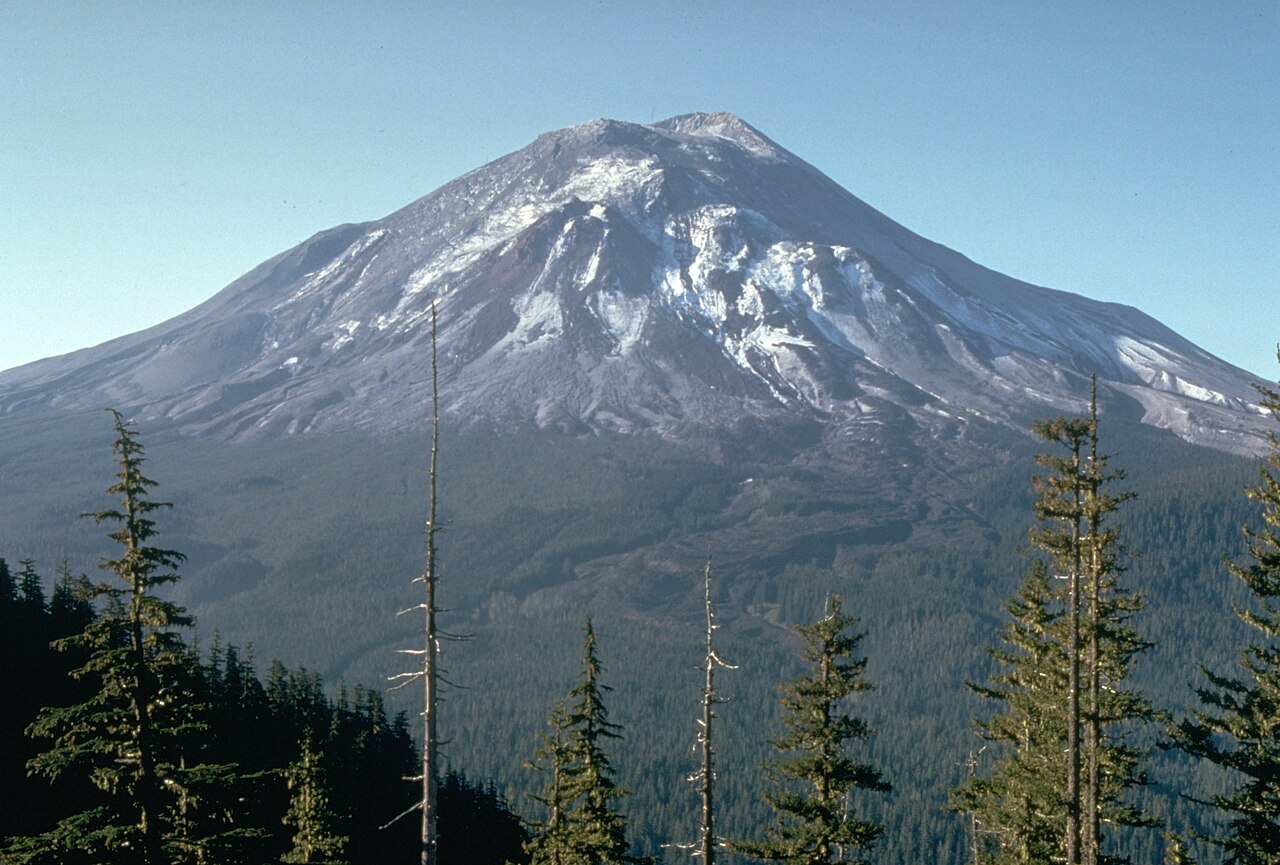
\includegraphics[width=\linewidth]{images/book1/g7-msh-before.jpg}

{\small 17 mai 1980, la veille.}
\end{minipage}\hfill
\begin{minipage}[b]{0.495\linewidth}\centering
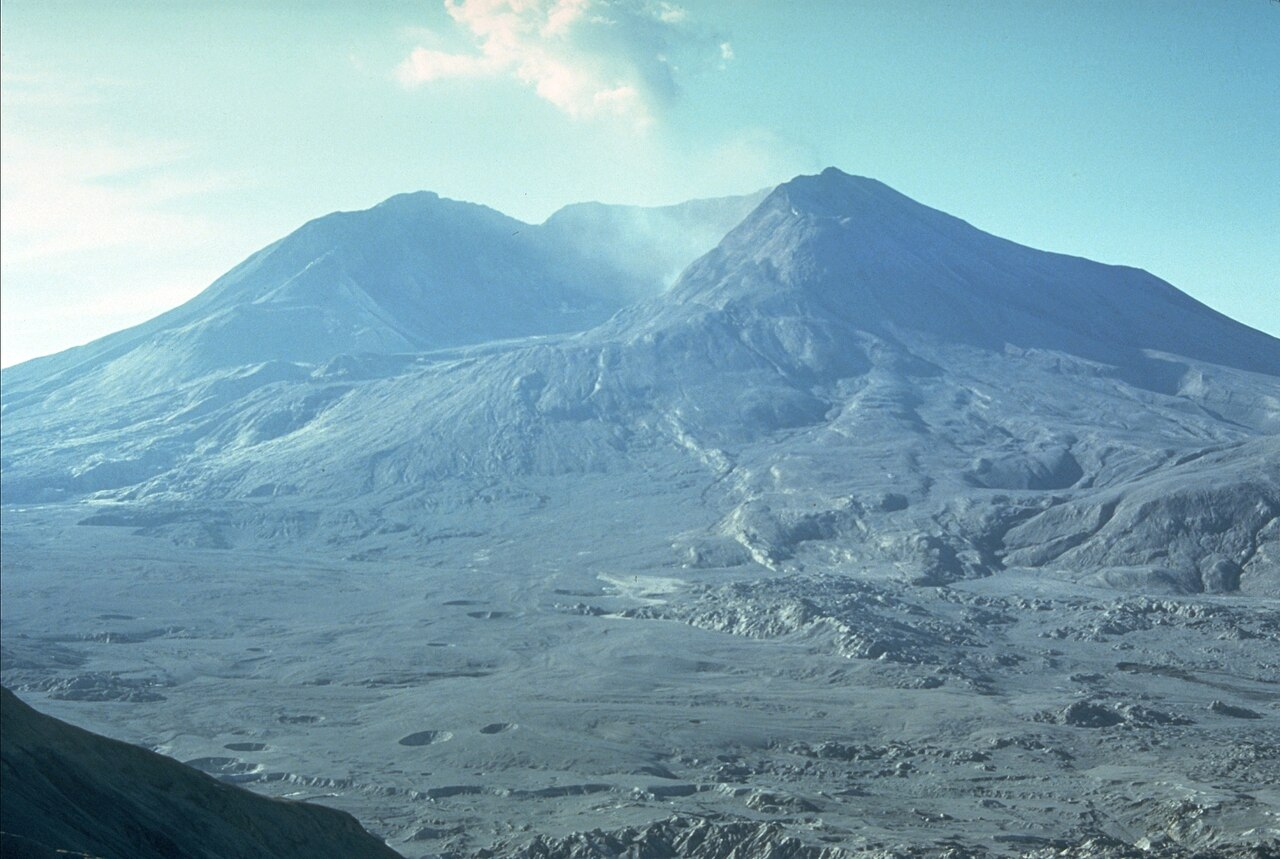
\includegraphics[width=\linewidth]{images/book1/g7-msh-after.jpg}

{\small 10 septembre 1980.}
\end{minipage}

{\small Le mont Saint Helens vu depuis Johnston Ridge, avant et après
l'\omterm{def:g4:volcanoes-earthquakes-first-look:eruption}{éruption} du 18~mai 1980. Le sommet et tout le flanc nord ont disparu~; un
\omterm{def:g7:volcanoes:vent}{cratère} ouvert vers le nord les a remplacés. Photographies~: Harry Glicken,
U.S. Geological Survey (domaine public, via Wikimedia Commons).}
% ledger: commons:msh-before, commons:msh-after, usgs:msh-lead-up, usgs:msh-may18
\label{fig:g7:volcanoes:st-helens}
\end{omfigure}

Dans ce chapitre, nous ouvrons un \omterm{def:g4:volcanoes-earthquakes-first-look:volcano}{volcan} pour voir ce qui provoque une
\omterm{def:g4:volcanoes-earthquakes-first-look:eruption}{éruption}~; nous découvrons pourquoi certains \omterm{def:g4:volcanoes-earthquakes-first-look:volcano}{volcans} déversent de
tranquilles \omterm{def:g1:landscapes-around-us:water}{rivières} de \omterm{def:g4:volcanoes-earthquakes-first-look:eruption}{lave} tandis que d'autres se font exploser~; et
nous regardons de nouveau la \omterm{def:g2:drawing-to-map:map}{carte} du monde, pour voir où se trouvent les
\omterm{def:g4:volcanoes-earthquakes-first-look:volcano}{volcans}, et pourquoi.

\begin{recall}
Un \emph{\omterm{def:g4:volcanoes-earthquakes-first-look:volcano}{volcan}} est un endroit où de la \omterm{def:g3:stones-pebbles-sand:rock}{roche} fondue venue des profondeurs
de la Terre sort à la surface, ainsi que la \omterm{def:g1:landscapes-around-us:landform}{colline} ou la \omterm{def:g1:landscapes-around-us:landform}{montagne} qu'elle
y construit. Pendant une \emph{\omterm{def:g4:volcanoes-earthquakes-first-look:eruption}{éruption}}, il projette de la \omterm{def:g4:volcanoes-earthquakes-first-look:eruption}{lave}, des
cendres et des gaz (\cref{ch:g4:volcanoes-earthquakes-first-look}). Sous la
\omterm{def:g6:inside-the-earth:layers}{croûte}, le \omterm{def:g6:inside-the-earth:layers}{manteau} est fait de \omterm{def:g3:stones-pebbles-sand:rock}{roche} chaude et solide, bien qu'elle puisse
se déformer très lentement (\cref{ch:g6:inside-the-earth}). Le basalte et le
granite sont des \omterm{def:g6:rocks-and-minerals:rock-families}{roches ignées}~: ils se forment quand de la \omterm{def:g3:stones-pebbles-sand:rock}{roche} fondue
refroidit et durcit (\cref{ch:g6:rocks-and-minerals}). L'enveloppe externe
de la Terre est découpée en \omterm{def:g7:plate-tectonics:plate}{plaques} qui se déplacent de quelques
centimètres par an~; leurs bords sont les \omterm{def:g7:plate-tectonics:plate-boundary}{limites de plaques}
(\cref{ch:g7:plate-tectonics}).
\end{recall}

\section{À l'intérieur d'un volcan}

Le \omterm{def:g6:inside-the-earth:layers}{manteau} est solide. Pourtant, en quelques endroits, loin sous la
surface, une petite partie de la \omterm{def:g3:stones-pebbles-sand:rock}{roche} fond. La \omterm{def:g3:stones-pebbles-sand:rock}{roche} fondue est plus
légère que la \omterm{def:g3:stones-pebbles-sand:rock}{roche} solide qui l'entoure~: elle monte donc lentement, en se
faufilant par des fissures, comme une goutte d'huile qui remonte dans
l'eau.
% ledger: usgs:hawaii-hotspot (magma lighter than the surrounding rock, rises)

\begin{definition}[Magma]\label{def:g7:volcanoes:magma}
Le \emph{magma}\index{magma} est de la \omterm{def:g3:stones-pebbles-sand:rock}{roche} fondue en profondeur. C'est un
liquide chaud qui peut aussi transporter des cristaux et, dissous en lui,
des gaz comme la vapeur d'eau et le dioxyde de carbone. Le magma qui sort à
la surface s'appelle la \omterm{def:g4:volcanoes-earthquakes-first-look:eruption}{lave}~; en sortant, il perd la plus grande partie de
ses gaz.
\end{definition}

Le \omterm{def:g7:volcanoes:magma}{magma} qui monte s'arrête souvent en chemin, à quelques kilomètres sous
la surface, et s'accumule dans une grande poche. Il y attend, parfois
pendant des siècles, avant qu'une \omterm{def:g4:volcanoes-earthquakes-first-look:eruption}{éruption} n'en vide une partie.

\begin{definition}[Chambre magmatique]\label{def:g7:volcanoes:magma-chamber}
Une \emph{chambre magmatique}\index{chambre magmatique} est un grand espace
dans les \omterm{def:g3:stones-pebbles-sand:rock}{roches} situées sous un \omterm{def:g4:volcanoes-earthquakes-first-look:volcano}{volcan}, à quelques kilomètres de
profondeur, où le \omterm{def:g7:volcanoes:magma}{magma} s'accumule avant une \omterm{def:g4:volcanoes-earthquakes-first-look:eruption}{éruption}.
\end{definition}

\begin{definition}[Bouche éruptive et cratère]\label{def:g7:volcanoes:vent}
Une \emph{bouche éruptive}\index{bouche eruptive@bouche éruptive} est une
ouverture à la surface par laquelle sortent le \omterm{def:g7:volcanoes:magma}{magma}, les gaz et les
cendres. Un \emph{cratère}\index{cratere@cratère} est le creux en forme de
cuvette qui entoure une bouche éruptive, en général au sommet du \omterm{def:g4:volcanoes-earthquakes-first-look:volcano}{volcan}.
\end{definition}

\begin{omfigure}
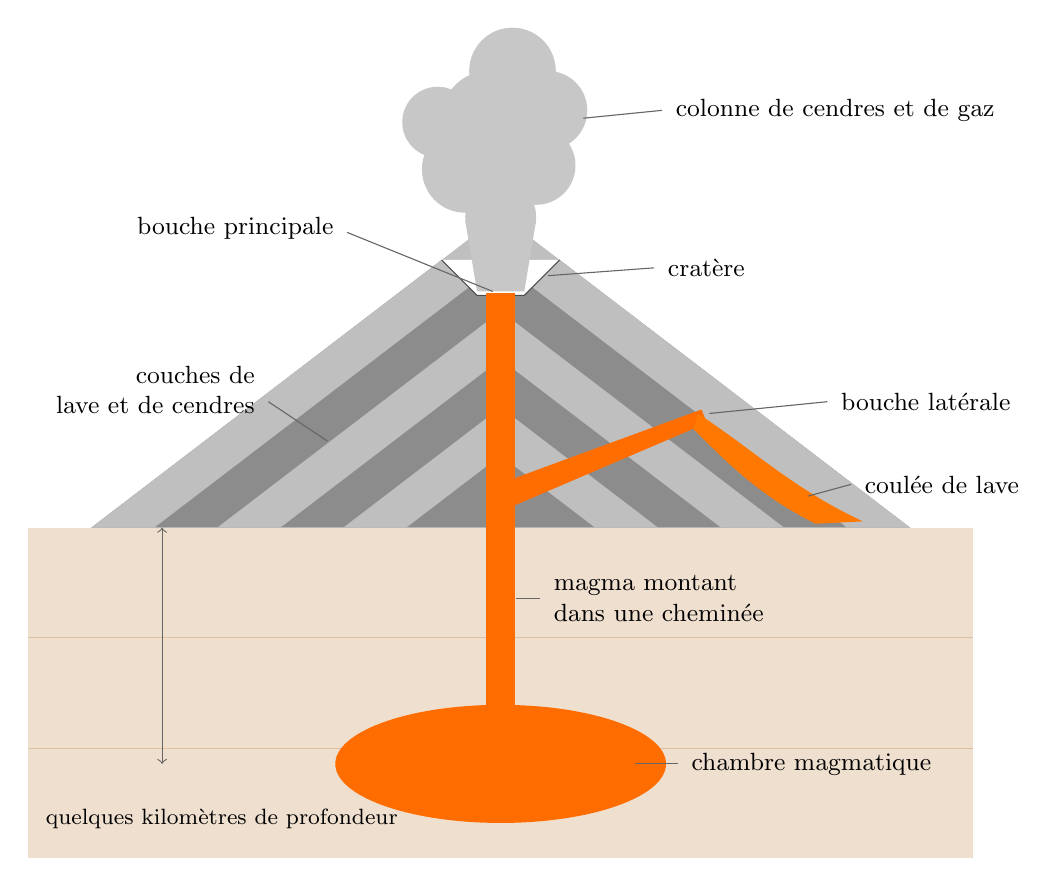
\begin{tikzpicture}[font=\small, x=1cm, y=1cm]
  % rocks below the volcano
  \fill[brown!25] (-6,-4.2) rectangle (6,0);
  \draw[brown!50] (-6,-1.4) -- (6,-1.4) (-6,-2.8) -- (6,-2.8);
  % the cone, built of layers of lava (dark) and ash (light)
  \fill[black!45] (-5.2,0) -- (-0.75,3.4) -- (0.75,3.4) -- (5.2,0) -- cycle;
    % layers dipping outwards, parallel to the flanks (slope 3.4/4.45)
  \foreach \k/\c in {0/black!25, 2/black!25, 4/black!25} {
    \pgfmathsetmacro{\xa}{-5.2+0.8*\k}\pgfmathsetmacro{\xb}{-5.2+0.8*(\k+1)}
    \pgfmathsetmacro{\ya}{(-0.18-\xa)*3.4/4.45}\pgfmathsetmacro{\yb}{(-0.18-\xb)*3.4/4.45}
    \fill[\c] (\xa,0) -- (-0.18,\ya) -- (-0.18,\yb) -- (\xb,0) -- cycle;
    \fill[\c] (-\xa,0) -- (0.18,\ya) -- (0.18,\yb) -- (-\xb,0) -- cycle;
  }
  % the crater at the top
  \fill[white] (-0.75,3.4) -- (-0.3,2.95) -- (0.3,2.95) -- (0.75,3.4) -- cycle;
  \draw[black!70] (-0.75,3.4) -- (-0.3,2.95) -- (0.3,2.95) -- (0.75,3.4);
  % magma chamber and the pipe up to the vent
  \fill[orange!85!red] (0,-3.0) ellipse (2.1 and 0.75);
  \fill[orange!85!red] (-0.18,-2.4) rectangle (0.18,2.98);
  % a side branch to a small side vent
  \fill[orange!85!red] (0.1,0.6) -- (2.55,1.5) -- (2.62,1.33) -- (0.1,0.25) -- cycle;
  % lava flow down the right flank, from the side vent
  \fill[orange!95!red] (2.5,1.45) .. controls (3.2,1.0) and (3.7,0.5) .. (4.6,0.08)
    -- (4.0,0.05) .. controls (3.3,0.4) and (2.9,0.8) .. (2.45,1.25) -- cycle;
  % ash column and gas
    \fill[black!22] (-0.3,3.0) -- (0.3,3.0) -- (0.45,3.9) -- (-0.45,3.9) -- cycle;
  \foreach \x/\y/\r in {0/3.95/0.45, -0.45/4.55/0.55, 0.45/4.6/0.5, -0.15/5.2/0.6,
                        0.6/5.3/0.5, -0.8/5.15/0.45, 0.15/5.8/0.55}
    \fill[black!22] (\x,\y) circle (\r);
  % labels
  \node[anchor=west] at (2.1,5.3) {colonne de cendres et de gaz};
  \draw[black!60] (2.05,5.3) -- (1.05,5.2);
  \node[anchor=west] at (2.0,3.3) {cratère};
  \draw[black!60] (1.95,3.3) -- (0.6,3.2);
  \node[anchor=east] at (-2.0,3.8) {bouche principale};
  \draw[black!60] (-1.95,3.75) -- (-0.1,3.0);
  \node[anchor=west] at (4.2,1.6) {bouche latérale};
  \draw[black!60] (4.15,1.6) -- (2.65,1.45);
  \node[anchor=west] at (4.5,0.55) {coulée de lave};
  \draw[black!60] (4.45,0.55) -- (3.9,0.4);
  \node[anchor=east, align=right] at (-3.0,1.75) {couches de\\lave et de cendres};
  \draw[black!60] (-2.95,1.6) -- (-2.2,1.1);
  \node[anchor=west, align=left] at (0.55,-0.9) {magma montant\\dans une cheminée};
  \draw[black!60] (0.5,-0.9) -- (0.2,-0.9);
  \node[anchor=west] at (2.3,-3.0) {chambre magmatique};
  \draw[black!60] (2.25,-3.0) -- (1.7,-3.0);
  \node[anchor=west, align=left, font=\footnotesize] at (-5.9,-3.7) {quelques kilomètres de profondeur};
  \draw[black!60, <->] (-4.3,0) -- (-4.3,-3.0);
\end{tikzpicture}

{\small Un \omterm{def:g4:volcanoes-earthquakes-first-look:volcano}{volcan} ouvert (un dessin, pas à l'échelle). Le \omterm{def:g7:volcanoes:magma}{magma} s'accumule
dans la \omterm{def:g7:volcanoes:magma-chamber}{chambre magmatique} et monte par une cheminée jusqu'à la \omterm{def:g7:volcanoes:vent}{bouche}
principale, au fond du \omterm{def:g7:volcanoes:vent}{cratère}~; une branche atteint une \omterm{def:g7:volcanoes:vent}{bouche} latérale
sur le flanc. Chaque \omterm{def:g4:volcanoes-earthquakes-first-look:eruption}{éruption} ajoute au cône une couche de \omterm{def:g4:volcanoes-earthquakes-first-look:eruption}{lave} ou de
cendres.}
\label{fig:g7:volcanoes:cutaway}
\end{omfigure}

La même \omterm{def:g3:stones-pebbles-sand:rock}{roche} fondue porte donc deux noms. En profondeur, c'est du
\emph{\omterm{def:g7:volcanoes:magma}{magma}}~; une fois sortie d'une \omterm{def:g7:volcanoes:vent}{bouche éruptive}, c'est de la
\emph{\omterm{def:g4:volcanoes-earthquakes-first-look:eruption}{lave}}. La différence n'est pas qu'une affaire de mots~: le \omterm{def:g7:volcanoes:magma}{magma}
contient encore ses gaz, tandis que la \omterm{def:g4:volcanoes-earthquakes-first-look:eruption}{lave} en a perdu la plus grande
partie dans l'air. Nous verrons que ces gaz décident du type d'\omterm{def:g4:volcanoes-earthquakes-first-look:eruption}{éruption}
d'un \omterm{def:g4:volcanoes-earthquakes-first-look:volcano}{volcan}.

Quelle est sa température~? Les scientifiques de l'Observatoire
volcanologique d'Hawaï mesurent la \omterm{def:g4:volcanoes-earthquakes-first-look:eruption}{lave} à sa sortie des \omterm{def:g7:volcanoes:vent}{bouches} du
Kilauea, l'un des \omterm{def:g4:volcanoes-earthquakes-first-look:volcano}{volcans} d'Hawaï~: environ \qty{1170}{\degreeCelsius}. La
\omterm{def:g3:stones-pebbles-sand:rock}{roche} chaude rougeoie, et la couleur de cette lueur dépend de sa
température~: des caméras spéciales lisent de loin la température d'une
coulée en mesurant les couleurs de sa lueur. Même l'œil s'en fait une idée
approximative, comme le montre le tableau.
% ledger: usgs:kilauea-temp, usgs:pyrometer

\begin{center}
\small
\begin{tabular}{|l|c|}
\hline
\textbf{couleur de la \omterm{def:g3:stones-pebbles-sand:rock}{roche} incandescente} & \textbf{température} \\
\hline
jaune & environ 1000 à \qty{1200}{\degreeCelsius} \\
orange & environ 800 à \qty{1000}{\degreeCelsius} \\
rouge & environ 600 à \qty{800}{\degreeCelsius} \\
\hline
\end{tabular}
\end{center}
% ledger: usgs:kilauea-temp

\begin{remark}[Une peau qui refroidit en une seconde]\label{rem:g7:volcanoes:skin}
% ledger: usgs:kilauea-temp
Quand la \omterm{def:g4:volcanoes-earthquakes-first-look:eruption}{lave} rencontre l'air, sa surface se refroidit de centaines de
degrés chaque seconde~: une peau sombre se forme aussitôt sur la \omterm{def:g3:stones-pebbles-sand:rock}{roche}
incandescente. Sous cette peau, la \omterm{def:g4:volcanoes-earthquakes-first-look:eruption}{lave} reste chaude longtemps. À Hawaï,
de la \omterm{def:g4:volcanoes-earthquakes-first-look:eruption}{lave} a coulé dans des tunnels, sous son propre toit durci, sur
\qty{10}{km}, d'une \omterm{def:g7:volcanoes:vent}{bouche} jusqu'à la \omterm{def:g2:water-on-earth:ocean}{mer}, et elle a encore atteint le
rivage à environ \qty{1140}{\degreeCelsius}~: seulement une trentaine de
degrés de moins qu'à la \omterm{def:g7:volcanoes:vent}{bouche}.
\end{remark}

\begin{omfigure}
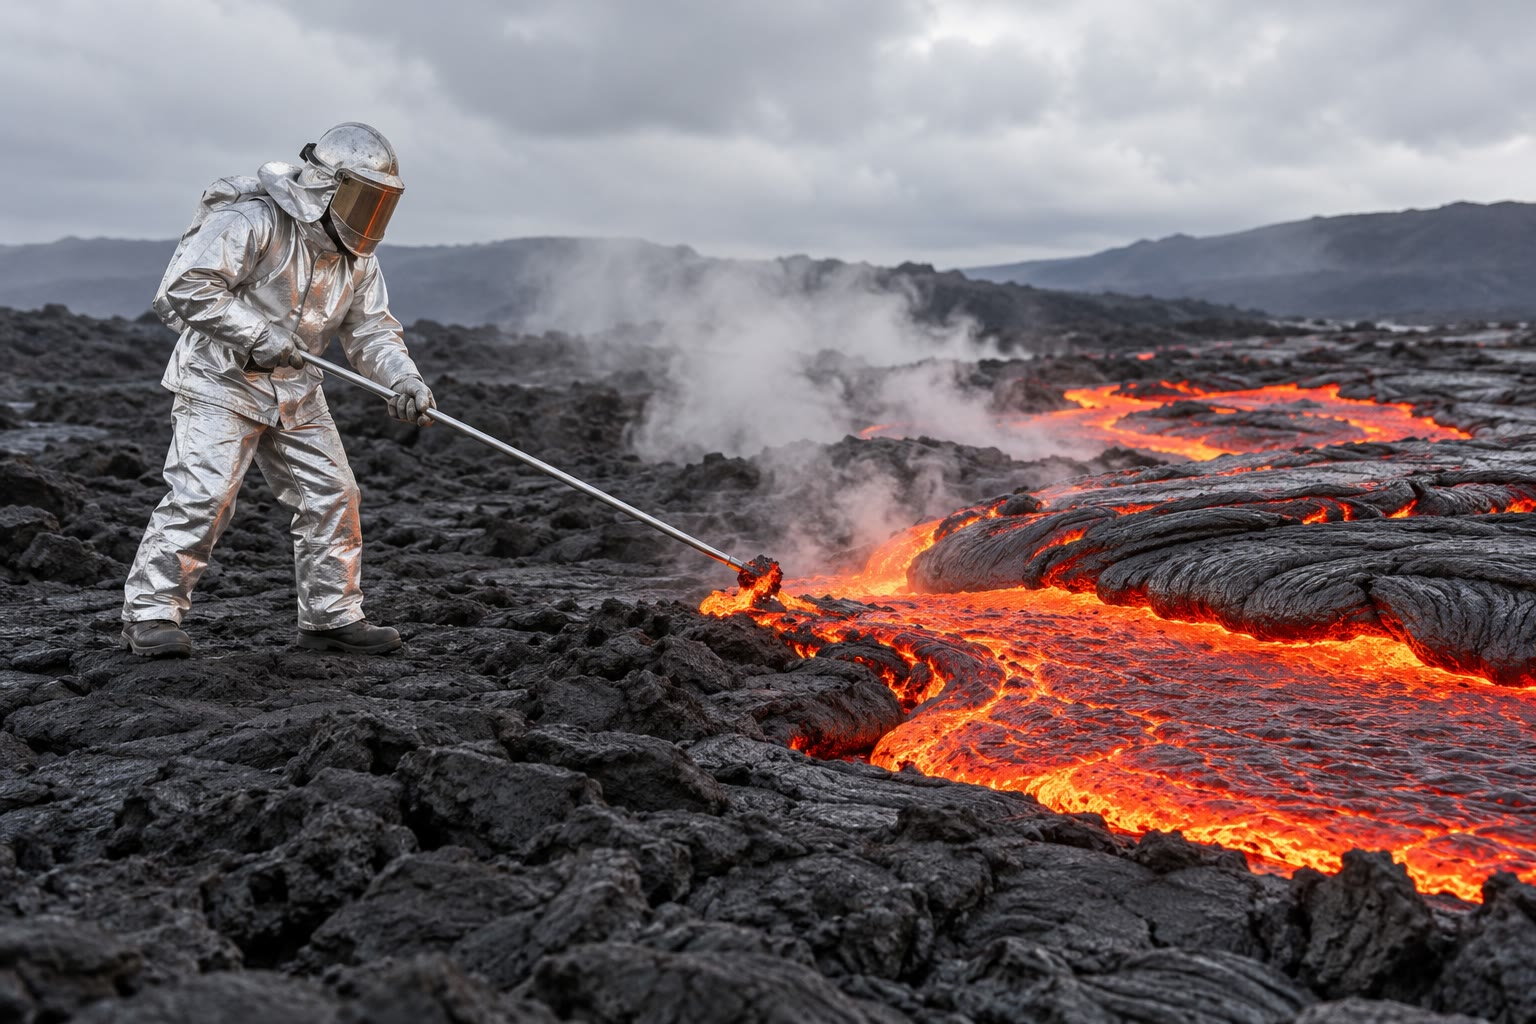
\includegraphics[width=0.6\linewidth]{images/book1/ai/g7-volcanologist.jpg}

{\small Une volcanologue en combinaison réfléchissant la chaleur prélève un
échantillon de \omterm{def:g4:volcanoes-earthquakes-first-look:eruption}{lave} avec une longue perche d'acier (illustration générée
par IA d'une scène générique). Seuls des scientifiques formés, avec ce
genre d'équipement, s'approchent de la \omterm{def:g4:volcanoes-earthquakes-first-look:eruption}{lave} qui coule~; tous les autres
regardent depuis les endroits autorisés par les autorités.}
\label{fig:g7:volcanoes:volcanologist}
\end{omfigure}

\section{Deux façons d'entrer en éruption}

Le mont Saint Helens s'est fait exploser. Les \omterm{def:g4:volcanoes-earthquakes-first-look:volcano}{volcans} d'Hawaï, au
contraire, déversent en général une \omterm{def:g4:volcanoes-earthquakes-first-look:eruption}{lave} qui s'écoule le long de leurs
pentes. Les géologues classent les \omterm{def:g4:volcanoes-earthquakes-first-look:eruption}{éruptions} en deux sortes.

\begin{definition}[Éruptions effusives et explosives]\label{def:g7:volcanoes:eruption-types}
Dans une \emph{éruption effusive}\index{eruption effusive@éruption effusive},
le \omterm{def:g7:volcanoes:magma}{magma} sort tranquillement sous forme de \omterm{def:g4:volcanoes-earthquakes-first-look:eruption}{lave}, qui s'écoule loin de la
\omterm{def:g7:volcanoes:vent}{bouche}, parfois sur des kilomètres, ou jaillit en fontaines de gouttes
incandescentes. Dans une
\emph{éruption explosive}\index{eruption explosive@éruption explosive}, le
\omterm{def:g7:volcanoes:magma}{magma} est réduit en morceaux par ses propres gaz~: une colonne de cendres,
de gaz et de blocs de \omterm{def:g3:stones-pebbles-sand:rock}{roche} est projetée haut dans le ciel.
\end{definition}

\begin{omfigure}
\begin{minipage}[t]{0.49\linewidth}\centering
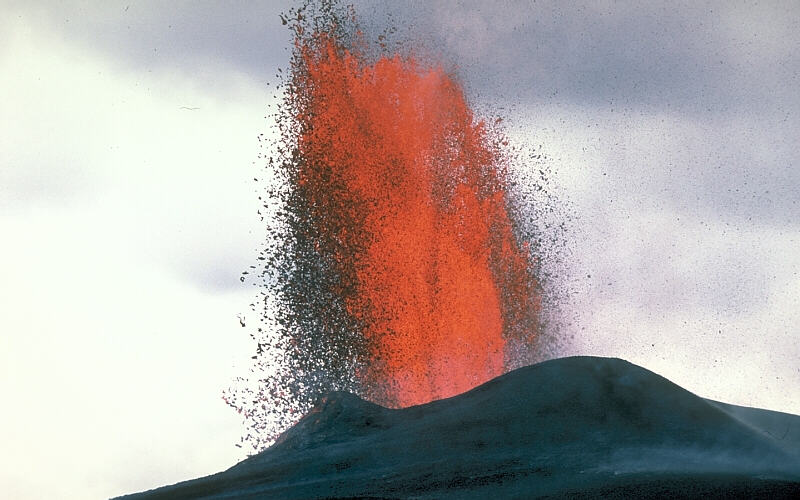
\includegraphics[height=4.5cm]{images/book1/g7-lava-fountain.jpg}

{\small Effusive~: une fontaine de \omterm{def:g4:volcanoes-earthquakes-first-look:eruption}{lave} au Kilauea, à Hawaï, en 1983.
Photographie~: J.~D. Griggs, USGS.}
\end{minipage}\hfill
\begin{minipage}[t]{0.49\linewidth}\centering
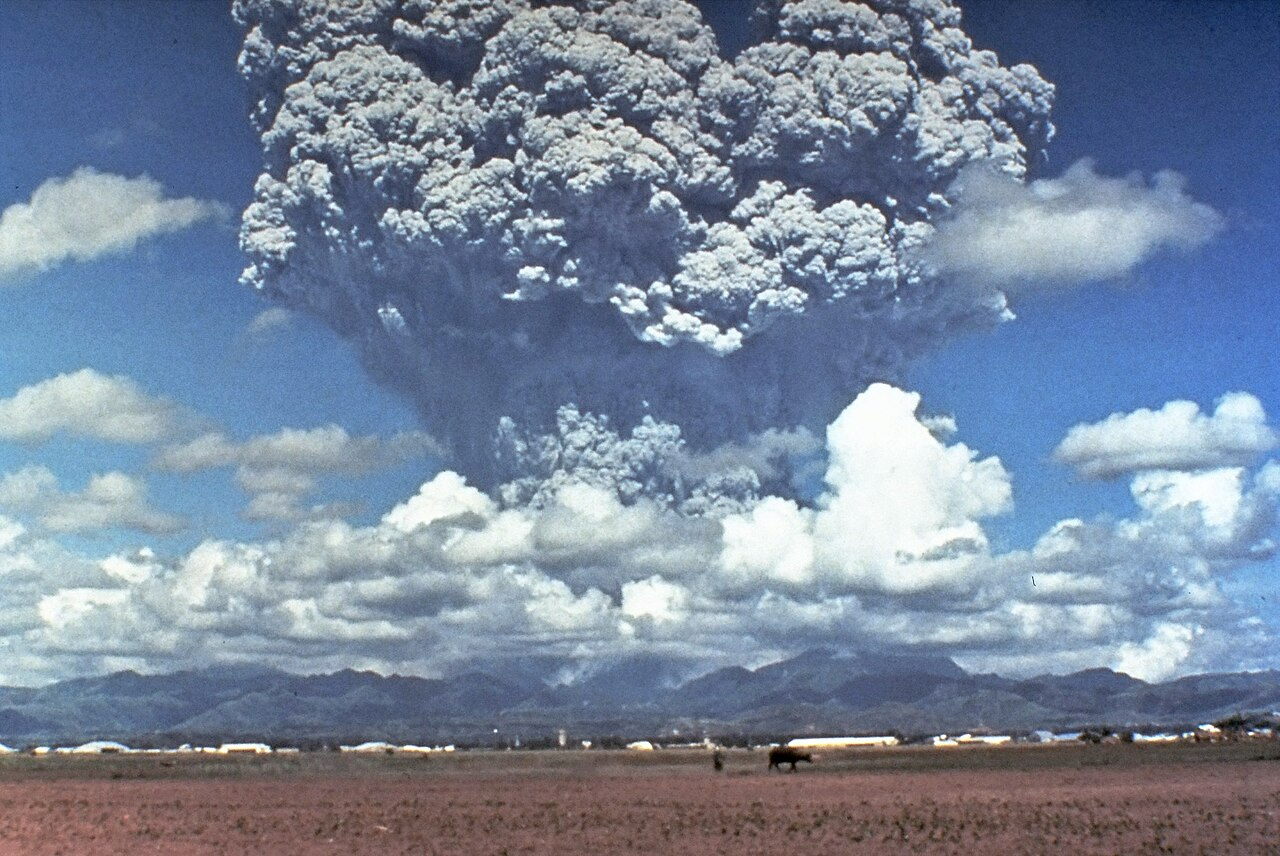
\includegraphics[height=4.5cm]{images/book1/g7-pinatubo.jpg}

{\small Explosive~: la colonne éruptive du mont Pinatubo, aux Philippines,
le 12~juin 1991. Photographie~: Dave Harlow, USGS.}
\end{minipage}\par\medskip


{\small Les deux photographies sont dans le domaine public (via Wikimedia
Commons).}
% ledger: commons:lava-fountain, commons:pinatubo
\label{fig:g7:volcanoes:two-photos}
\end{omfigure}

Qu'est-ce qui fait la différence~? Deux choses~: la fluidité du \omterm{def:g7:volcanoes:magma}{magma}, et
la quantité de gaz qu'il contient.

\textbf{Fluide ou visqueux.} Certains \omterm{def:g7:volcanoes:magma}{magmas} sont fluides, presque comme du
miel tiède~: c'est le cas du \omterm{def:g7:volcanoes:magma}{magma} qui refroidit en basalte sombre, comme à
Hawaï. D'autres \omterm{def:g7:volcanoes:magma}{magmas} sont épais et visqueux, comme du miel froid ou du
dentifrice. Dans un \omterm{def:g7:volcanoes:magma}{magma} fluide, les bulles de gaz montent facilement et
s'échappent à la surface, quelques-unes à la fois. Dans un \omterm{def:g7:volcanoes:magma}{magma} visqueux,
les bulles sont piégées.

\textbf{Peu ou beaucoup de gaz.} Une bouteille d'eau gazeuse contient
beaucoup de gaz dissous dans l'eau, maintenu là par la pression à
l'intérieur de la bouteille fermée~; on ne le voit pas. Ouvre la bouteille,
et la pression chute~: des bulles apparaissent partout, et si la bouteille
a été secouée, la mousse jaillit. Le \omterm{def:g7:volcanoes:magma}{magma}, en profondeur, contient lui
aussi des gaz dissous sous une forte pression. Pendant qu'il monte, la
pression baisse et les gaz sortent de la solution sous forme de bulles.
% ledger: usgs:volcanic-gases

Assemblons les deux. Un \omterm{def:g7:volcanoes:magma}{magma} fluide et pauvre en gaz laisse partir ses
bulles et sort sous forme de \omterm{def:g4:volcanoes-earthquakes-first-look:eruption}{lave} qui coule~: l'\omterm{def:g4:volcanoes-earthquakes-first-look:eruption}{éruption} est effusive. Un
\omterm{def:g7:volcanoes:magma}{magma} visqueux et riche en gaz garde ses bulles jusqu'à ce qu'elles
gonflent au point de déchiqueter le \omterm{def:g7:volcanoes:magma}{magma}~: l'\omterm{def:g4:volcanoes-earthquakes-first-look:eruption}{éruption} est explosive. Les
lambeaux de \omterm{def:g7:volcanoes:magma}{magma} mousseux se figent dans l'air en cendres et en ponce, une
\omterm{def:g3:stones-pebbles-sand:rock}{roche} si pleine de bulles qu'elle peut flotter.

\begin{example}[Pinatubo, 1991~: le soda éventé et le soda secoué]\label{ex:g7:volcanoes:pinatubo}
% ledger: usgs:pinatubo-1991
En juin~1991, le premier \omterm{def:g7:volcanoes:magma}{magma} a atteint la surface du mont Pinatubo, aux
Philippines. En montant, il avait perdu la plus grande partie de ses gaz,
«~comme une bouteille de soda éventée~», selon les mots des scientifiques
qui l'observaient. Il est sorti lentement et s'est entassé en un dôme
au-dessus de la \omterm{def:g7:volcanoes:vent}{bouche}~: pas d'explosion. Puis, le 12~juin, un \omterm{def:g7:volcanoes:magma}{magma}
encore plein de gaz a atteint la surface et a explosé --- la colonne de la
photographie ci-dessus. Le 15~juin, un \omterm{def:g7:volcanoes:magma}{magma} encore plus riche en gaz est
arrivé, et le \omterm{def:g4:volcanoes-earthquakes-first-look:volcano}{volcan} a connu l'une des plus grandes \omterm{def:g4:volcanoes-earthquakes-first-look:eruption}{éruptions} du
\textsc{xx}\textsuperscript{e}~siècle~: il a projeté plus de cinq
kilomètres cubes de \omterm{def:g3:stones-pebbles-sand:rock}{roche} et de cendres, son \omterm{def:g4:clouds-rain-snow:cloud}{nuage} de cendres est monté à
\qty{35}{km} de haut, et le sommet de la \omterm{def:g1:landscapes-around-us:landform}{montagne} s'est effondré en un
creux de \qty{2.5}{km} de large. Le même \omterm{def:g4:volcanoes-earthquakes-first-look:volcano}{volcan}, la même semaine~: ce sont
les gaz qui ont fait la différence.
\end{example}

La forme d'un \omterm{def:g4:volcanoes-earthquakes-first-look:volcano}{volcan} garde la mémoire de ses \omterm{def:g4:volcanoes-earthquakes-first-look:eruption}{éruptions}. Une \omterm{def:g4:volcanoes-earthquakes-first-look:eruption}{lave} fluide
coule loin avant de durcir~: couche après couche, elle construit une large
\omterm{def:g1:landscapes-around-us:landform}{montagne} aux pentes douces, en forme de bouclier de guerrier posé sur le
sol~: un \emph{\omterm{def:g4:volcanoes-earthquakes-first-look:volcano}{volcan} bouclier}. Le Mauna Loa, à Hawaï, en est un. La \omterm{def:g4:volcanoes-earthquakes-first-look:eruption}{lave}
visqueuse et les cendres s'entassent près de la \omterm{def:g7:volcanoes:vent}{bouche}, en un cône raide
fait de couches de \omterm{def:g4:volcanoes-earthquakes-first-look:eruption}{lave} et de cendres~: un \emph{stratovolcan}
(\emph{strata} veut dire «~couches~»). Le mont Saint Helens et le
Pinatubo en sont deux exemples.

\begin{omfigure}
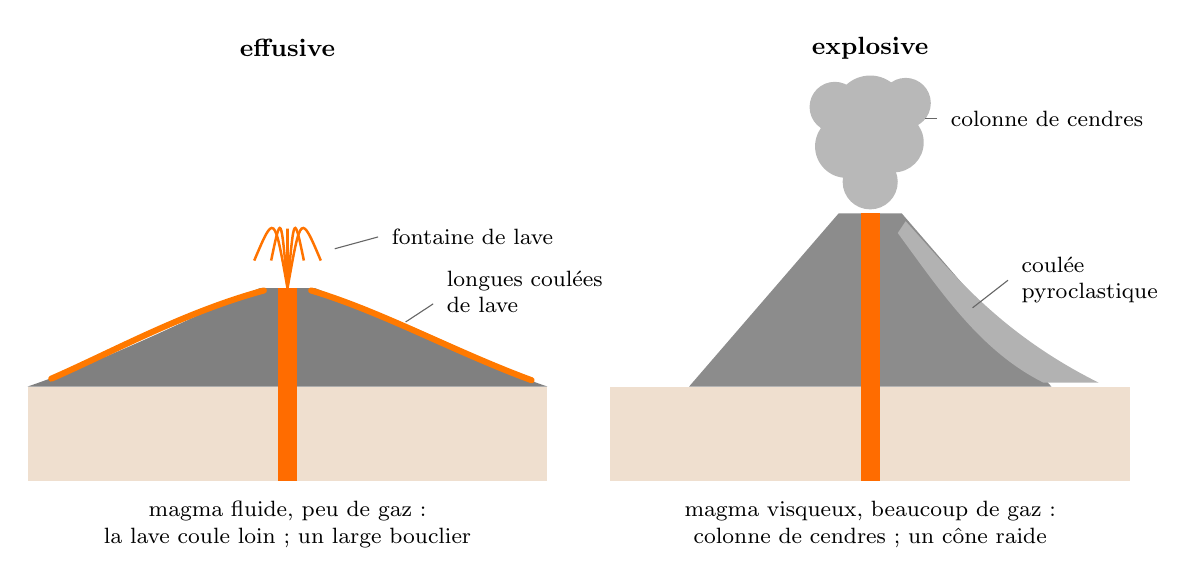
\begin{tikzpicture}[font=\small, x=1cm, y=1cm]
  % --- left: effusive, a shield
  \begin{scope}
    \fill[brown!25] (-3.3,-1.2) rectangle (3.3,0);
    \fill[black!50] (-3.3,0) .. controls (-2.0,0.45) and (-1.0,1.0) .. (-0.35,1.25)
      -- (0.35,1.25) .. controls (1.0,1.0) and (2.0,0.45) .. (3.3,0) -- cycle;
    \fill[orange!85!red] (-0.12,-1.2) rectangle (0.12,1.25);
    % fountain
    \foreach \a in {-25,-12,0,12,25}
      \draw[orange!90!red, line width=0.9pt] (0,1.25) .. controls ({0.4*sin(\a)},2.2) .. ({1.0*sin(\a)},1.6);
    % lava flows far down the gentle slopes
    \draw[orange!95!red, line width=2.2pt, line cap=round] (0.3,1.22) .. controls (1.2,0.95) and (2.1,0.45) .. (3.1,0.08);
    \draw[orange!95!red, line width=2.2pt, line cap=round] (-0.3,1.22) .. controls (-1.3,0.95) and (-2.2,0.45) .. (-3.0,0.1);
    \node[font=\small\bfseries] at (0,4.3) {effusive};
    \node[align=center, font=\footnotesize] at (0,-1.75) {magma fluide, peu de gaz~:\\la lave coule loin~; un large bouclier};
    \node[anchor=west, font=\footnotesize] at (1.2,1.9) {fontaine de lave};
    \draw[black!60] (1.15,1.9) -- (0.6,1.75);
    \node[anchor=west, font=\footnotesize, align=left] at (1.9,1.2) {longues coulées\\de lave};
    \draw[black!60] (1.85,1.05) -- (1.5,0.82);
  \end{scope}
  % --- right: explosive, a steep cone
  \begin{scope}[xshift=7.4cm]
    \fill[brown!25] (-3.3,-1.2) rectangle (3.3,0);
    \fill[black!45] (-2.3,0) -- (-0.4,2.2) -- (0.4,2.2) -- (2.3,0) -- cycle;
    \fill[orange!85!red] (-0.12,-1.2) rectangle (0.12,2.2);
    \foreach \x/\y/\r in {0/2.6/0.35, -0.3/3.05/0.4, 0.3/3.1/0.38, 0/3.5/0.45, -0.45/3.55/0.32, 0.45/3.6/0.32}
      \fill[black!28] (\x,\y) circle (\r);
    % pyroclastic flow down the flank
    \fill[black!30] (0.45,2.1) .. controls (1.0,1.5) and (1.6,0.7) .. (2.9,0.05)
      -- (2.2,0.05) .. controls (1.4,0.45) and (0.9,1.2) .. (0.35,1.95) -- cycle;
    \node[font=\small\bfseries] at (0,4.3) {explosive};
    \node[align=center, font=\footnotesize] at (0,-1.75) {magma visqueux, beaucoup de gaz~:\\colonne de cendres~; un cône raide};
    \node[anchor=west, font=\footnotesize] at (0.9,3.4) {colonne de cendres};
    \draw[black!60] (0.85,3.4) -- (0.7,3.4);
    \node[anchor=west, font=\footnotesize, align=left] at (1.8,1.35) {coulée\\pyroclastique};
    \draw[black!60] (1.75,1.35) -- (1.3,1.0);
  \end{scope}
\end{tikzpicture}

{\small Les deux sortes d'\omterm{def:g4:volcanoes-earthquakes-first-look:eruption}{éruption} et les \omterm{def:g4:volcanoes-earthquakes-first-look:volcano}{volcans} qu'elles construisent
(dessins, pas à l'échelle).}
\label{fig:g7:volcanoes:two-kinds}
\end{omfigure}

\begin{method}[Effusive ou explosive~? Quatre indices]\label{met:g7:volcanoes:clues}
Pour reconnaître, d'après une description ou une photographie, le type
d'\omterm{def:g4:volcanoes-earthquakes-first-look:eruption}{éruption} d'un \omterm{def:g4:volcanoes-earthquakes-first-look:volcano}{volcan}, cherche ces indices.
\begin{enumerate}
  \item \emph{Qu'est-ce qui sort~?} De la \omterm{def:g4:volcanoes-earthquakes-first-look:eruption}{lave} qui coule ou jaillit en
        fontaines~: effusive. Une colonne de cendres, des blocs de \omterm{def:g3:stones-pebbles-sand:rock}{roche}
        projetés~: explosive.
  \item \emph{La forme du \omterm{def:g4:volcanoes-earthquakes-first-look:volcano}{volcan}.} Une large \omterm{def:g1:landscapes-around-us:landform}{montagne} aux pentes douces~:
        \omterm{def:g4:volcanoes-earthquakes-first-look:eruption}{éruptions} surtout effusives. Un cône raide~: souvent explosives.
  \item \emph{Le \omterm{def:g7:volcanoes:magma}{magma}.} Fluide, peu de gaz~: effusive. Visqueux, beaucoup
        de gaz~: explosive.
  \item \emph{Les \omterm{def:g3:stones-pebbles-sand:rock}{roches} laissées.} Des coulées de \omterm{def:g4:volcanoes-earthquakes-first-look:eruption}{lave} sombres et
        massives~: effusive. Des couches de cendres et de ponce~:
        explosive.
\end{enumerate}
\end{method}

\begin{example}[Utiliser les indices]\label{ex:g7:volcanoes:clues}
Une voyageuse décrit un \omterm{def:g4:volcanoes-earthquakes-first-look:volcano}{volcan}~: «~une énorme \omterm{def:g1:landscapes-around-us:landform}{montagne} aux formes
doucement arrondies, des coulées de \omterm{def:g4:volcanoes-earthquakes-first-look:eruption}{lave} noire partout sur ses pentes,
certaines vieilles de quelques années seulement~». L'indice~2 (pentes
douces) et l'indice~4 (coulées de \omterm{def:g4:volcanoes-earthquakes-first-look:eruption}{lave} sombres) indiquent tous deux des
\omterm{def:g7:volcanoes:eruption-types}{éruptions effusives}~: c'est un \omterm{def:g4:volcanoes-earthquakes-first-look:volcano}{volcan} bouclier, comme le Mauna Loa.
\end{example}

\begin{inthelab}[Un volcan en bouteille (en classe, avec l'enseignant)]
L'enseignant prend deux bouteilles fermées d'eau gazeuse. L'une est restée
posée~; l'autre a été doucement secouée. Toutes deux sont ouvertes dehors,
au-dessus d'une bassine, tournées loin de tout le monde. La bouteille
restée posée siffle et laisse monter quelques bulles~; la bouteille
secouée éclate en une mousse qui jaillit. Quelle bouteille ressemble au
\omterm{def:g7:volcanoes:magma}{magma} d'Hawaï, laquelle à celui du Pinatubo~? Ensuite, on laisse tomber un
morceau de ponce et un \omterm{def:g3:stones-pebbles-sand:pebble}{galet} dans un bol d'eau~: la ponce flotte.
Regarde-la à la loupe~: elle est pleine de trous, les bulles de gaz figées
dans la \omterm{def:g3:stones-pebbles-sand:rock}{roche} quand le \omterm{def:g7:volcanoes:magma}{magma} a éclaté.
\end{inthelab}

\section{Ce qui sort d'un volcan}

Une \omterm{def:g4:volcanoes-earthquakes-first-look:eruption}{éruption} projette bien plus que de la \omterm{def:g4:volcanoes-earthquakes-first-look:eruption}{lave}~: des gaz, des cendres, des
blocs de \omterm{def:g3:stones-pebbles-sand:rock}{roche} et, dans les pires cas, des avalanches de cendres
brûlantes.

Le gaz le plus abondant, de loin, est la vapeur d'eau. Les grandes
\omterm{def:g4:volcanoes-earthquakes-first-look:eruption}{éruptions} libèrent d'énormes quantités de gaz en peu de temps~: en une
seule journée de 1991, le Pinatubo aurait envoyé plus de 250~millions de
tonnes de gaz dans la haute atmosphère.
% ledger: usgs:volcanic-gases

\begin{definition}[Coulée pyroclastique]\label{def:g7:volcanoes:pyroclastic-flow}
Une \emph{coulée pyroclastique}\index{coulee pyroclastique@coulée pyroclastique}
est une avalanche rapide de gaz brûlants, de cendres et de morceaux de
\omterm{def:g3:stones-pebbles-sand:rock}{roche}, des grains de poussière aux blocs, qui dévale les pentes d'un \omterm{def:g4:volcanoes-earthquakes-first-look:volcano}{volcan}
pendant une \omterm{def:g7:volcanoes:eruption-types}{éruption explosive}. (\emph{Pyro} veut dire «~feu~» et
\emph{clastique} veut dire «~fait de morceaux brisés~».)
\end{definition}

Les \omterm{def:g7:volcanoes:pyroclastic-flow}{coulées pyroclastiques} se déplacent en général à plus de
\qty{80}{km/h}, et les \omterm{def:g3:stones-pebbles-sand:rock}{roches} et les gaz qu'elles contiennent sont en
général entre 200 et \qty{700}{\degreeCelsius}. Elles suivent le plus
souvent les \omterm{def:g1:landscapes-around-us:landform}{vallées}, comme l'eau, et elles renversent, brûlent ou
ensevelissent presque tout sur leur passage. Le 18~mai 1980, les \omterm{def:g7:volcanoes:pyroclastic-flow}{coulées
pyroclastiques} du mont Saint Helens ont filé à 80 à \qty{130}{km/h}, à une
température d'au moins \qty{700}{\degreeCelsius}, et ont atteint
\qty{8}{km} du \omterm{def:g7:volcanoes:vent}{cratère}.
% ledger: usgs:pyroclastic-flows, usgs:msh-flows, usgs:msh-reach

Le tableau résume les produits d'un \omterm{def:g4:volcanoes-earthquakes-first-look:volcano}{volcan}.

\begin{center}
\small
\begin{tabular}{|p{0.2\linewidth}|p{0.4\linewidth}|p{0.3\linewidth}|}
\hline
\textbf{produit} & \textbf{ce que c'est} & \textbf{le danger} \\
\hline
coulée de \omterm{def:g4:volcanoes-earthquakes-first-look:eruption}{lave} & \omterm{def:g3:stones-pebbles-sand:rock}{roche} fondue qui coule sur le sol, puis durcit & brûle et ensevelit ce qu'elle rencontre, mais en général assez lente pour que l'on puisse s'écarter \\
\hline
cendres & minuscules morceaux de \omterm{def:g3:stones-pebbles-sand:rock}{roche} et de verre, soufflés dans l'air & tombent loin~; les toits s'effondrent sous leur poids~; elles endommagent les avions \\
\hline
bombes volcaniques & blocs de \omterm{def:g4:volcanoes-earthquakes-first-look:eruption}{lave} projetés, qui durcissent en vol & écrasent ce qu'elles touchent, près de la \omterm{def:g7:volcanoes:vent}{bouche} \\
\hline
gaz & surtout de la vapeur d'eau, puis du dioxyde de carbone et du dioxyde de soufre & certains sont toxiques~; le dioxyde de carbone s'accumule dans les creux \\
\hline
\omterm{def:g7:volcanoes:pyroclastic-flow}{coulée pyroclastique} & une avalanche de cendres, de \omterm{def:g3:stones-pebbles-sand:rock}{roches} et de gaz brûlants & la plus meurtrière~: trop rapide et trop chaude pour qu'on lui échappe \\
\hline
coulée de boue & cendres et \omterm{def:g3:stones-pebbles-sand:rock}{roches} mêlées à l'eau de \omterm{def:g4:clouds-rain-snow:precipitation}{pluie} ou de \omterm{def:g4:clouds-rain-snow:precipitation}{neige} fondue & dévale les \omterm{def:g1:landscapes-around-us:landform}{vallées}, parfois loin du \omterm{def:g4:volcanoes-earthquakes-first-look:volcano}{volcan} \\
\hline
\end{tabular}
\end{center}
% ledger: usgs:lava-flows, usgs:volcanic-gases, usgs:pyroclastic-flows, usgs:pinatubo-1991, usgs:msh-flows

\begin{method}[Combien de temps faut-il~?]\label{met:g7:volcanoes:time}
Pour trouver combien de temps met un objet qui se déplace à une vitesse
connue pour parcourir une distance, divise la distance par la vitesse~:
\[
\text{durée} = \frac{\text{distance}}{\text{vitesse}}.
\]
Avec une distance en kilomètres et une vitesse en kilomètres par heure, la
durée s'obtient en heures~; multiplie par 60 pour obtenir des minutes.
\end{method}

\begin{example}[La course contre une coulée pyroclastique]\label{ex:g7:volcanoes:race}
Une \omterm{def:g7:volcanoes:pyroclastic-flow}{coulée pyroclastique} qui avance à \qty{120}{km/h} se dirige vers un
village situé \qty{6}{km} plus bas dans la \omterm{def:g1:landscapes-around-us:landform}{vallée}. Elle met
$6 \div 120 = 0.05$~heure, soit $0.05 \times 60 = 3$~minutes. Trois
minutes~: personne ne peut sortir de la \omterm{def:g1:landscapes-around-us:landform}{vallée} à temps, ni en courant ni
même en voiture. Les gens ne sont en sécurité que s'ils sont partis
\emph{avant} l'\omterm{def:g4:volcanoes-earthquakes-first-look:eruption}{éruption}.
\end{example}

\begin{remark}[Les coulées de boue~: le danger qui vient après]\label{rem:g7:volcanoes:mudflows}
% ledger: usgs:msh-flows, usgs:pinatubo-lahars
Une \omterm{def:g4:volcanoes-earthquakes-first-look:eruption}{éruption} laisse les pentes couvertes de cendres meubles. Quand la \omterm{def:g4:clouds-rain-snow:precipitation}{pluie}
tombe dessus, ou quand la chaleur fait fondre la \omterm{def:g4:clouds-rain-snow:precipitation}{neige} et la glace du
sommet, les cendres se transforment en coulées de boue qui dévalent les
\omterm{def:g1:landscapes-around-us:landform}{vallées}. Le 18~mai 1980, les coulées de boue du mont Saint Helens ont
endommagé 27~ponts et près de 200~maisons. Autour du Pinatubo, les fortes
\omterm{def:g4:clouds-rain-snow:precipitation}{pluies} des années suivantes ont transformé les cendres en coulées de boue
géantes qui ont enseveli des villages entiers~: elles ont fait plus de
dégâts que l'\omterm{def:g4:volcanoes-earthquakes-first-look:eruption}{éruption} elle-même.
\end{remark}


\section{Où sont les volcans~?}

La Smithsonian Institution, à Washington, tient une liste de tous les
\omterm{def:g4:volcanoes-earthquakes-first-look:volcano}{volcans} qui ont connu une \omterm{def:g4:volcanoes-earthquakes-first-look:eruption}{éruption} au cours des 12\,000 dernières
années~: il y en a 1\,214, sur terre et sous la \omterm{def:g2:water-on-earth:ocean}{mer}. Pour chacun, la liste
indique où il se trouve par rapport aux \omterm{def:g7:plate-tectonics:plate}{plaques}. La \omterm{def:g2:drawing-to-map:map}{carte} ci-dessous les
colore de cette façon.
% ledger: data:gvp (counts computed in figdata/grade-7/volcano_settings.py)

\begin{omfigure}
\begin{tikzpicture}
\begin{axis}[ommap, width=\linewidth, xtick={-180,-90,...,180}, ytick={-60,0,60},
  legend style={at={(0.02,0.04)}, anchor=south west, font=\scriptsize,
  fill=white, fill opacity=0.85, text opacity=1, draw=black!40}, legend cell align=left]
\addplot[fill=omLithAlluv, draw=black!45, line width=0.2pt, forget plot] table {figdata/out/shared-geo-land.dat};
\addplot[omRidge!60, line width=0.5pt, forget plot] table {figdata/out/shared-geo-school-ridge.dat};
\addplot[omTrench!60, line width=0.5pt, forget plot] table {figdata/out/shared-geo-school-subduction.dat};
\addplot[only marks, mark=triangle*, mark size=1.3pt, omTrench, forget plot] table {figdata/out/grade-7-volcano_settings-map-sub.dat};
\addplot[only marks, mark=triangle*, mark size=1.3pt, omRidge, forget plot] table {figdata/out/grade-7-volcano_settings-map-rift.dat};
\addplot[only marks, mark=*, mark size=1.4pt, orange!90!black, forget plot] table {figdata/out/grade-7-volcano_settings-map-intra.dat};
\addlegendimage{only marks, mark=triangle*, mark size=1.6pt, omTrench}
\addlegendentry{là où une plaque s'enfonce sous une autre}
\addlegendimage{only marks, mark=triangle*, mark size=1.6pt, omRidge}
\addlegendentry{là où des plaques s'écartent}
\addlegendimage{only marks, mark=*, mark size=1.6pt, orange!90!black}
\addlegendentry{à l'intérieur d'une plaque}
\end{axis}
\end{tikzpicture}

{\small Les \omterm{def:g4:volcanoes-earthquakes-first-look:volcano}{volcans} actifs au cours des 12\,000 dernières années, colorés
selon l'endroit où ils se trouvent. Lignes pâles~: les limites où des
\omterm{def:g7:plate-tectonics:plate}{plaques} s'écartent (en rouge) et celles où une \omterm{def:g7:plate-tectonics:plate}{plaque} s'enfonce sous une
autre (en bleu). Données~: Global Volcanism Program de la Smithsonian
Institution~; limites d'après P.~Bird (2003)~; côtes d'après Natural
Earth.}
% ledger: data:gvp, data:pb2002, data:ne-land
\label{fig:g7:volcanoes:map}
\end{omfigure}

\begin{omfigure}
\begin{tikzpicture}
  \begin{axis}[xbar, width=0.72\linewidth, height=3.6cm, bar width=8pt,
      xmin=0, xmax=1000, ymin=-0.6, ymax=3.6, y dir=reverse,
      ytick={0,...,3}, yticklabels={où une plaque s'enfonce sous une autre, où des plaques s'écartent, à l'intérieur d'une plaque, inconnu},
      xlabel={nombre de volcans},
      axis x line=bottom, axis y line=left, axis line style={-},
      tick label style={font=\scriptsize}, label style={font=\small},
      nodes near coords, nodes near coords style={font=\scriptsize, anchor=west},
      point meta=explicit symbolic, enlarge y limits=false, clip=false]
    \addplot[fill=black!30, draw=black!60] table[x=n, y=idx, meta=n] {figdata/out/grade-7-volcano_settings.dat};
  \end{axis}
\end{tikzpicture}

{\small Combien des 1\,214 \omterm{def:g4:volcanoes-earthquakes-first-look:volcano}{volcans} se trouvent dans chaque situation.}
% ledger: data:gvp (figdata/grade-7/volcano_settings.py, main table)
\label{fig:g7:volcanoes:counts}
\end{omfigure}

\begin{proposition}[La plupart des volcans se trouvent sur des limites de plaques]\label{prop:g7:volcanoes:where}
% ledger: data:gvp (counts computed in figdata/grade-7/volcano_settings.py)
Sur les 1\,214 \omterm{def:g4:volcanoes-earthquakes-first-look:volcano}{volcans} actifs au cours des 12\,000 dernières années, 838
(69~\%) se trouvent là où une \omterm{def:g7:plate-tectonics:plate}{plaque} s'enfonce sous une autre et 221
(18~\%) là où des \omterm{def:g7:plate-tectonics:plate}{plaques} s'écartent~; 149 (12~\%) se trouvent à
l'intérieur d'une \omterm{def:g7:plate-tectonics:plate}{plaque}, loin de ses bords. Pour les 6 derniers (0.5~\%), la
situation est inconnue.
\end{proposition}

\textbf{Là où des \omterm{def:g7:plate-tectonics:plate}{plaques} s'écartent.} Le long des dorsales océaniques, et
dans des rifts comme celui qui est en train de déchirer l'Afrique de l'Est,
les \omterm{def:g7:plate-tectonics:plate}{plaques} s'éloignent l'une de l'autre. Du \omterm{def:g7:volcanoes:magma}{magma} monte du \omterm{def:g6:inside-the-earth:layers}{manteau} dans
les fissures qui s'élargissent et les remplit~: de la \omterm{def:g6:inside-the-earth:layers}{croûte} nouvelle se
forme. La plupart des dorsales sont sous la \omterm{def:g2:water-on-earth:ocean}{mer}, mais l'Islande se trouve
juste sur la dorsale médio-atlantique~: là, ces \omterm{def:g4:volcanoes-earthquakes-first-look:volcano}{volcans} se voient sur la
terre ferme. Leur \omterm{def:g7:volcanoes:magma}{magma} est surtout du basalte fluide, et leurs \omterm{def:g4:volcanoes-earthquakes-first-look:eruption}{éruptions}
sont surtout effusives.
% ledger: usgs:arc-magma, usgs:iceland, usgs:east-africa

\textbf{Là où une \omterm{def:g7:plate-tectonics:plate}{plaque} s'enfonce sous une autre.} Plus de deux \omterm{def:g4:volcanoes-earthquakes-first-look:volcano}{volcans}
sur trois se trouvent ici, le long de lignes qui suivent les bords de
l'\omterm{def:g2:water-on-earth:ocean}{océan} Pacifique --- la «~ceinture de feu~» --- et en quelques autres
endroits. En profondeur, le long de la \omterm{def:g7:plate-tectonics:plate}{plaque} qui s'enfonce, une partie de
la \omterm{def:g3:stones-pebbles-sand:rock}{roche} fond en partie~; les scientifiques discutent encore pour savoir
exactement quelle \omterm{def:g3:stones-pebbles-sand:rock}{roche} fond, la \omterm{def:g7:plate-tectonics:plate}{plaque} qui s'enfonce, la \omterm{def:g7:plate-tectonics:plate}{plaque} qui est
au-dessus, ou les deux. Le \omterm{def:g7:volcanoes:magma}{magma} qui monte là est souvent visqueux et
plein de gaz~: ce sont les \omterm{def:g4:volcanoes-earthquakes-first-look:volcano}{volcans} explosifs, comme le mont Saint Helens
et le Pinatubo. Les données le montrent~: sur les 660 cônes raides
(stratovolcans) de la liste, 564 --- soit 85~\% --- se trouvent là où une
\omterm{def:g7:plate-tectonics:plate}{plaque} s'enfonce sous une autre.
% ledger: usgs:arc-magma, data:gvp (figdata/grade-7/volcano_settings.py, part strato)

\textbf{À l'intérieur d'une \omterm{def:g7:plate-tectonics:plate}{plaque}.} Quelques \omterm{def:g4:volcanoes-earthquakes-first-look:volcano}{volcans} sont loin de toute
limite. Les plus célèbres sont ceux d'Hawaï, au milieu de l'\omterm{def:g2:water-on-earth:ocean}{océan}
Pacifique, à plus de \qty{3200}{km} du bord de \omterm{def:g7:plate-tectonics:plate}{plaque} le plus proche.
% ledger: usgs:hawaii-hotspot

\begin{definition}[Point chaud]\label{def:g7:volcanoes:hotspot}
Un \emph{point chaud}\index{point chaud} est un endroit, profond dans le
\omterm{def:g6:inside-the-earth:layers}{manteau}, qui reste chaud pendant des millions d'années et continue
d'alimenter en \omterm{def:g7:volcanoes:magma}{magma} des \omterm{def:g4:volcanoes-earthquakes-first-look:volcano}{volcans} de surface, même loin des bords des
\omterm{def:g7:plate-tectonics:plate}{plaques}.
\end{definition}

Le \omterm{def:g7:volcanoes:hotspot}{point chaud} reste où il est, tandis que la \omterm{def:g7:plate-tectonics:plate}{plaque} qui le surmonte se
déplace. Un \omterm{def:g4:volcanoes-earthquakes-first-look:volcano}{volcan} grandit au-dessus du \omterm{def:g7:volcanoes:hotspot}{point chaud}~; puis la \omterm{def:g7:plate-tectonics:plate}{plaque} en
mouvement l'emporte, et il s'éteint, tandis qu'un nouveau \omterm{def:g4:volcanoes-earthquakes-first-look:volcano}{volcan} grandit
derrière lui, au-dessus du \omterm{def:g7:volcanoes:hotspot}{point chaud}. Avec le temps, la \omterm{def:g7:plate-tectonics:plate}{plaque} porte
toute une ligne de \omterm{def:g4:volcanoes-earthquakes-first-look:volcano}{volcans}, les plus anciens étant les plus éloignés du
\omterm{def:g7:volcanoes:hotspot}{point chaud}. C'est exactement ce que l'on voit à Hawaï~: les \omterm{def:g3:stones-pebbles-sand:rock}{roches} les
plus anciennes de l'île de Kauai, à l'extrémité nord-ouest des îles
habitées, ont environ 5.5~millions d'années et sont profondément usées
par la \omterm{def:g4:clouds-rain-snow:precipitation}{pluie} et les vagues~; sur Big Island, à l'extrémité sud-est, les
\omterm{def:g3:stones-pebbles-sand:rock}{roches} les plus anciennes en surface ont moins de 0.7~million d'années, et
de la \omterm{def:g4:volcanoes-earthquakes-first-look:eruption}{lave} nouvelle sort encore.
% ledger: usgs:hawaii-hotspot

\begin{history}[Un géophysicien et une ligne d'îles]
% ledger: usgs:hawaii-hotspot
Pourquoi une chaîne d'îles volcaniques s'élèverait-elle au milieu de la
plus grande \omterm{def:g7:plate-tectonics:plate}{plaque} de la Terre~? En 1963, le géophysicien canadien J.~Tuzo
Wilson a proposé une réponse. Les îles d'Hawaï, a-t-il suggéré, forment
une ligne parce que la \omterm{def:g7:plate-tectonics:plate}{plaque} pacifique se déplace au-dessus d'une source
de chaleur profonde et fixe dans le \omterm{def:g6:inside-the-earth:layers}{manteau}, qui fait fondre en partie la
\omterm{def:g7:plate-tectonics:plate}{plaque} située au-dessus. S'il avait raison, les îles devaient être d'autant
plus anciennes et plus usées qu'elles sont loin des \omterm{def:g4:volcanoes-earthquakes-first-look:volcano}{volcans} actifs de Big
Island. Les âges de leurs \omterm{def:g3:stones-pebbles-sand:rock}{roches} montrent exactement cela. Une seule idée
expliquait à la fois la ligne et l'ordre des âges. (Wilson est aussi le
scientifique qui a découvert les \omterm{def:g7:plate-tectonics:plate-boundary}{limites transformantes}, où des \omterm{def:g7:plate-tectonics:plate}{plaques}
glissent l'une le long de l'autre.)
\end{history}

\begin{omfigure}
\begin{tikzpicture}[font=\small, x=1cm, y=1cm]
  % sea, plate and mantle
  \fill[omSea!45] (-6.2,0) rectangle (6.2,1.0);
  \fill[orange!12] (-6.2,-3.4) rectangle (6.2,-1.0);
  \fill[brown!35] (-6.2,-1.0) rectangle (6.2,0);
  \draw[omSea!80!black, line width=0.5pt] (-6.2,1.0) -- (6.2,1.0);
  \node[font=\footnotesize] at (-4.6,-0.5) {plaque pacifique};
  % the hotspot plume, fixed in the mantle, and the magma rising to the volcano
  \fill[orange!80!red] (4.0,-3.4) .. controls (3.6,-2.4) .. (3.75,-1.0) -- (4.25,-1.0) .. controls (4.4,-2.4) .. (4.0,-3.4) -- cycle;
  \node[anchor=west, align=left, font=\footnotesize] at (4.5,-2.5) {point chaud~: reste\\en place};
  % volcanoes rise from the sea floor; youngest over the hotspot
  \fill[black!55] (2.3,0) .. controls (3.2,1.2) .. (3.75,1.85) -- (4.25,1.85) .. controls (4.8,1.2) .. (5.7,0) -- cycle;
  \fill[orange!80!red] (3.93,-1.0) rectangle (4.07,1.85);
  \fill[black!45] (-0.4,0) .. controls (0.4,0.9) .. (0.9,1.3) -- (1.3,1.3) .. controls (1.8,0.9) .. (2.6,0) -- cycle;
  \fill[black!35] (-3.2,0) .. controls (-2.5,0.6) .. (-2.1,0.8) -- (-1.7,0.8) .. controls (-1.3,0.6) .. (-0.6,0) -- cycle;
  \fill[black!28] (-5.8,0) .. controls (-5.2,0.4) .. (-4.9,0.5) -- (-4.6,0.5) .. controls (-4.3,0.4) .. (-3.6,0) -- cycle;
  % labels
    \node[align=center, font=\footnotesize, anchor=south] at (4.3,1.95) {volcan actif\\(Big Island~: moins\\de 0.7 million d'années)};
  \node[align=center, font=\footnotesize, anchor=south] at (0.7,1.4) {île ancienne et usée\\(Kauai~: environ\\5.5 millions d'années)};
  \node[align=center, font=\footnotesize] at (-1.9,1.5) {volcan plus ancien,\\sous les vagues};
  \node[align=center, font=\footnotesize] at (-4.75,1.3) {encore plus ancien,\\qui s'enfonce};
  \node[font=\footnotesize] at (5.75,0.55) {mer};
  \node[font=\footnotesize] at (-4.3,-2.2) {manteau};
  % plate motion
  \draw[-{Stealth[length=3mm]}, line width=1.2pt] (2.2,-0.62) -- (-1.8,-0.62);
  \node[font=\footnotesize] at (0.2,-0.28) {la plaque se déplace vers le nord-ouest};
    \node[font=\footnotesize\bfseries] at (-5.8,-3.1) {NO};
  \node[font=\footnotesize\bfseries] at (5.8,-3.1) {SE};
\end{tikzpicture}

{\small Une \omterm{def:g7:plate-tectonics:plate}{plaque} qui se déplace au-dessus d'un \omterm{def:g7:volcanoes:hotspot}{point chaud} (un dessin, pas
à l'échelle~; les îles intermédiaires sont omises). Le \omterm{def:g4:volcanoes-earthquakes-first-look:volcano}{volcan} situé
au-dessus du \omterm{def:g7:volcanoes:hotspot}{point chaud} est jeune et actif~; la \omterm{def:g7:plate-tectonics:plate}{plaque} emporte les plus
anciens vers le nord-ouest, où ils s'éteignent, s'usent et finissent par
s'enfoncer sous les vagues.}
% ledger: usgs:hawaii-hotspot
\label{fig:g7:volcanoes:hotspot}
\end{omfigure}

\begin{omfigure}
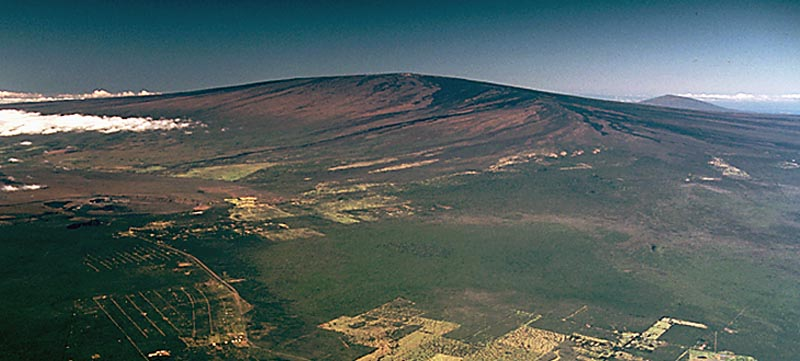
\includegraphics[width=0.8\linewidth]{images/book1/g7-mauna-loa.jpg}

{\small Le Mauna Loa, un \omterm{def:g4:volcanoes-earthquakes-first-look:volcano}{volcan} bouclier de Big Island, à Hawaï, vu
d'avion~: une immense \omterm{def:g1:landscapes-around-us:landform}{montagne} aux pentes douces, construite par des
milliers de coulées de \omterm{def:g4:volcanoes-earthquakes-first-look:eruption}{lave} fluide. Photographie~: J.~D. Griggs,
U.S. Geological Survey, 1985 (domaine public, via Wikimedia Commons).}
% ledger: commons:mauna-loa
\label{fig:g7:volcanoes:mauna-loa}
\end{omfigure}

\section{Vivre avec les volcans}

Beaucoup de gens vivent près des \omterm{def:g4:volcanoes-earthquakes-first-look:volcano}{volcans}~: environ 3~millions vivaient dans
la région du Pinatubo en 1991. Heureusement, une grande \omterm{def:g4:volcanoes-earthquakes-first-look:eruption}{éruption} donne
souvent des signes avant-coureurs. Le \omterm{def:g7:volcanoes:magma}{magma} qui monte écarte les \omterm{def:g3:stones-pebbles-sand:rock}{roches}~:
le sol se fissure et tremble avec de petits \omterm{def:g4:volcanoes-earthquakes-first-look:earthquake}{séismes}, les pentes gonflent,
des gaz s'échappent. Au mont Saint Helens, les premiers petits \omterm{def:g4:volcanoes-earthquakes-first-look:earthquake}{séismes} sont
arrivés le 16~mars 1980~; au 17~mai, il y en avait eu plus de 10\,000, et
le flanc nord avait gonflé vers l'extérieur d'au moins \qty{137}{m}. Les
scientifiques ont mesuré tout cela et la zone a été fermée~; malgré cela,
57~personnes sont mortes le 18~mai.
% ledger: usgs:msh-lead-up, usgs:msh-flows

Au Pinatubo, en 1991, les scientifiques qui surveillaient les \omterm{def:g4:volcanoes-earthquakes-first-look:earthquake}{séismes}, les
gaz et le gonflement du \omterm{def:g4:volcanoes-earthquakes-first-look:volcano}{volcan} ont donné l'alerte à temps~: les gens qui
vivaient près du \omterm{def:g4:volcanoes-earthquakes-first-look:volcano}{volcan} sont partis, et au moins 5\,000 vies ont été
sauvées.
% ledger: usgs:pinatubo-1991 (central Luzon home to about 3 million people)

\begin{remark}[Ne t'approche jamais d'un volcan en éruption]\label{rem:g7:volcanoes:safety}
Regarder une \omterm{def:g4:volcanoes-earthquakes-first-look:eruption}{éruption} n'est possible que depuis les endroits que les
autorités ont ouverts au public. Les gaz, les chutes de pierres, la \omterm{def:g6:inside-the-earth:layers}{croûte}
de \omterm{def:g4:volcanoes-earthquakes-first-look:eruption}{lave} fraîche qui cède sous les pieds et les \omterm{def:g7:volcanoes:pyroclastic-flow}{coulées pyroclastiques}
peuvent tuer, souvent sans prévenir. Les observatoires volcanologiques
publient ce que l'on peut visiter sans danger~: suis toujours leurs
consignes.
\end{remark}

\section{Exercices}

\begin{exercise}[$\star$]\label{exo:g7:volcanoes:1}
Associe chaque mot à sa définition~: \omterm{def:g7:volcanoes:magma}{magma}~; \omterm{def:g4:volcanoes-earthquakes-first-look:eruption}{lave}~; \omterm{def:g7:volcanoes:magma-chamber}{chambre magmatique}~;
\omterm{def:g7:volcanoes:vent}{bouche éruptive}~; \omterm{def:g7:volcanoes:vent}{cratère}. (a) Un creux en forme de cuvette au sommet d'un
\omterm{def:g4:volcanoes-earthquakes-first-look:volcano}{volcan}. (b) De la \omterm{def:g3:stones-pebbles-sand:rock}{roche} fondue en profondeur. (c) Une ouverture par
laquelle sort le \omterm{def:g7:volcanoes:magma}{magma}. (d) De la \omterm{def:g3:stones-pebbles-sand:rock}{roche} fondue sortie à la surface. (e) Une
grande poche de \omterm{def:g7:volcanoes:magma}{magma} à quelques kilomètres sous un \omterm{def:g4:volcanoes-earthquakes-first-look:volcano}{volcan}.
\end{exercise}

\begin{exercise}[$\star$]\label{exo:g7:volcanoes:2}
Effusive ou explosive~? (a) Des \omterm{def:g1:landscapes-around-us:water}{rivières} de \omterm{def:g4:volcanoes-earthquakes-first-look:eruption}{lave} incandescente coulent sur
une pente douce. (b) Une colonne de cendres monte à \qty{35}{km} dans le
ciel. (c) Une fontaine de gouttes incandescentes jaillit d'une fissure.
(d) Une avalanche de cendres et de gaz brûlants dévale une \omterm{def:g1:landscapes-around-us:landform}{vallée}.
\end{exercise}

\begin{exercise}[$\star$]\label{exo:g7:volcanoes:3}
Vrai ou faux~? Corrige les phrases fausses. (a) Le \omterm{def:g7:volcanoes:magma}{magma} et la \omterm{def:g4:volcanoes-earthquakes-first-look:eruption}{lave} sont
deux noms de la même \omterm{def:g3:stones-pebbles-sand:rock}{roche} fondue, en profondeur et à la surface. (b) Le
gaz volcanique le plus abondant est le dioxyde de carbone. (c) Une \omterm{def:g7:volcanoes:pyroclastic-flow}{coulée
pyroclastique} est une \omterm{def:g1:landscapes-around-us:water}{rivière} de \omterm{def:g4:volcanoes-earthquakes-first-look:eruption}{lave} liquide. (d) Les \omterm{def:g4:volcanoes-earthquakes-first-look:volcano}{volcans} d'Hawaï se
trouvent sur une \omterm{def:g7:plate-tectonics:plate-boundary}{limite de plaques}.
\end{exercise}

\begin{exercise}[$\star$]\label{exo:g7:volcanoes:4}
Utilise le tableau des couleurs de la lueur. (a) Une \omterm{def:g4:volcanoes-earthquakes-first-look:eruption}{lave} rougeoie en
jaune~: donne sa température. (b) Une coulée qui durcit rougeoie en rouge
sombre~: donne sa température. (c) Une photographie montre de la \omterm{def:g4:volcanoes-earthquakes-first-look:eruption}{lave}
orange au front d'une coulée et de la \omterm{def:g4:volcanoes-earthquakes-first-look:eruption}{lave} jaune près de la \omterm{def:g7:volcanoes:vent}{bouche}. Où
fait-il le plus chaud~? Pourquoi~?
\end{exercise}

\begin{exercise}[$\star\star$]\label{exo:g7:volcanoes:5}
Utilise le diagramme en bâtons des 1\,214 \omterm{def:g4:volcanoes-earthquakes-first-look:volcano}{volcans}. (a) Combien de \omterm{def:g4:volcanoes-earthquakes-first-look:volcano}{volcans}
se trouvent sur une \omterm{def:g7:plate-tectonics:plate-boundary}{limite de plaques} (là où des \omterm{def:g7:plate-tectonics:plate}{plaques} s'écartent, ou là
où l'une s'enfonce sous l'autre)~? (b) Quel pourcentage de tous les \omterm{def:g4:volcanoes-earthquakes-first-look:volcano}{volcans}
cela représente-t-il~? (c) Vérifie que les quatre pourcentages de la
proposition font au total environ 100~\%.
\end{exercise}

\begin{exercise}[$\star\star$]\label{exo:g7:volcanoes:6}
Sur les 660 cônes raides (stratovolcans) de la liste, 564 se trouvent là où
une \omterm{def:g7:plate-tectonics:plate}{plaque} s'enfonce sous une autre, 62 là où des \omterm{def:g7:plate-tectonics:plate}{plaques} s'écartent et 33
à l'intérieur d'une \omterm{def:g7:plate-tectonics:plate}{plaque}. (a) Trouve le pourcentage des cônes raides qui
se trouvent là où une \omterm{def:g7:plate-tectonics:plate}{plaque} s'enfonce sous une autre. (b) Combien de
cônes raides reste-t-il pour la situation «~inconnue~»~? (c) Utilise les
quatre indices~: à quelles \omterm{def:g4:volcanoes-earthquakes-first-look:eruption}{éruptions} faut-il s'attendre le long de la
ceinture de feu~?
\end{exercise}

\begin{exercise}[$\star\star$]\label{exo:g7:volcanoes:7}
Au Kilauea, la \omterm{def:g4:volcanoes-earthquakes-first-look:eruption}{lave} sort de la \omterm{def:g7:volcanoes:vent}{bouche} à environ \qty{1170}{\degreeCelsius}.
Dans un tunnel de \omterm{def:g4:volcanoes-earthquakes-first-look:eruption}{lave}, elle a atteint la \omterm{def:g2:water-on-earth:ocean}{mer}, à \qty{10}{km}, à environ
\qty{1140}{\degreeCelsius}. (a) De combien de degrés s'est-elle
refroidie~? (b) Combien de degrés cela fait-il par kilomètre~? (c) À l'air
libre, la \omterm{def:g4:volcanoes-earthquakes-first-look:eruption}{lave} se refroidit en surface de centaines de degrés par seconde.
Explique pourquoi la \omterm{def:g4:volcanoes-earthquakes-first-look:eruption}{lave} du tunnel est restée si chaude.
\end{exercise}

\begin{exercise}[$\star\star$]\label{exo:g7:volcanoes:8}
Les \omterm{def:g3:stones-pebbles-sand:rock}{roches} les plus anciennes de Kauai ont environ 5.5~millions d'années~;
celles de Big Island, moins de 0.7~million d'années. (a) Quelle île est la
plus ancienne~? D'au moins combien de millions d'années~? (b) Quelle île
est la plus usée~? Pourquoi~? (c) Quelle île se trouve au-dessus du \omterm{def:g7:volcanoes:hotspot}{point
chaud} aujourd'hui~? (d) Kauai se trouve au nord-ouest de Big Island. Dans
quelle direction la \omterm{def:g7:plate-tectonics:plate}{plaque} pacifique emporte-t-elle les îles~?
\end{exercise}

\begin{exercise}[$\star\star$]\label{exo:g7:volcanoes:9}
Les îles d'Hawaï sont à plus de \qty{3200}{km} de la \omterm{def:g7:plate-tectonics:plate-boundary}{limite de plaques} la
plus proche. (a) Pourquoi est-ce surprenant pour des \omterm{def:g4:volcanoes-earthquakes-first-look:volcano}{volcans}~? (b) Explique
en trois ou quatre phrases d'où vient leur \omterm{def:g7:volcanoes:magma}{magma}. (c) Sur la \omterm{def:g2:drawing-to-map:map}{carte} des
\omterm{def:g4:volcanoes-earthquakes-first-look:volcano}{volcans}, de quelle couleur sont-ils~?
\end{exercise}

\begin{exercise}[$\star\star$]\label{exo:g7:volcanoes:10}
En juin~1991, le premier \omterm{def:g7:volcanoes:magma}{magma} du Pinatubo est sorti tranquillement~; trois
jours plus tard, un autre \omterm{def:g7:volcanoes:magma}{magma} a explosé. À l'aide des deux bouteilles
d'eau gazeuse, explique la différence. Lequel des deux \omterm{def:g7:volcanoes:magma}{magmas} avait perdu
ses gaz en montant~?
\end{exercise}

\begin{exercise}[$\star\star\star$]\label{exo:g7:volcanoes:11}
Un village se trouve \qty{10}{km} en aval d'un \omterm{def:g4:volcanoes-earthquakes-first-look:volcano}{volcan}, dans une \omterm{def:g1:landscapes-around-us:landform}{vallée}.
(a) Une \omterm{def:g7:volcanoes:pyroclastic-flow}{coulée pyroclastique} avance à \qty{80}{km/h}. Combien de minutes
lui faudrait-il pour atteindre le village~? (b) Même question à
\qty{130}{km/h}. (c) Une famille a besoin de 20~minutes pour partir en
voiture. Explique pourquoi l'alerte doit être donnée avant le début de
l'\omterm{def:g4:volcanoes-earthquakes-first-look:eruption}{éruption}, et non quand on voit la coulée.
\end{exercise}

\begin{exercise}[$\star\star\star$]\label{exo:g7:volcanoes:12}
Les cendres du mont Saint Helens ont fait une fois le tour de la Terre
entière en 15~jours. Un degré de \omterm{def:g6:latitude-longitude:latitude}{latitude} mesure environ \qty{111}{km}, et
un tour complet fait 360~degrés. (a) Quelle est la longueur approximative
d'un tour complet de la Terre, en kilomètres~? Arrondis au millier. (b)
Combien de kilomètres les cendres ont-elles parcourus par jour, en
moyenne~? (c) Combien de kilomètres par heure cela fait-il~? (d) Les
cendres sont-elles portées par le vent ou par leur propre vitesse~?
Explique.
% ledger: usgs:msh-may18, rmg:latitude-def
\end{exercise}

\section{Problème~: Le jour où la montagne a perdu son sommet}

\begin{problem}[{Problème du week-end --- les signes avant-coureurs du mont Saint Helens,
l'éruption du 18~mai 1980, et la part de la montagne qui a disparu}]
\label{pb:g7:volcanoes:1}
% ledger: usgs:msh-heights, usgs:msh-lead-up, usgs:msh-may18, usgs:msh-flows, usgs:msh-reach, usgs:msh-dome, usgs:msh-faq-loss, data:gvp, tht:everest

Le mont Saint Helens se trouve dans le nord-ouest des États-Unis. Utilise
les photographies du début du chapitre, la \omterm{def:g2:drawing-to-map:map}{carte} des \omterm{def:g4:volcanoes-earthquakes-first-look:volcano}{volcans} et les
nombres ci-dessous, mesurés par l'U.S. Geological Survey.

\medskip
\noindent\textbf{Partie I --- Avant l'éruption.}
\begin{enumerate}
  \item Les premiers petits \omterm{def:g4:volcanoes-earthquakes-first-look:earthquake}{séismes} sont arrivés le 16~mars 1980~; la grande
        \omterm{def:g4:volcanoes-earthquakes-first-look:eruption}{éruption}, le 18~mai. Combien de jours se sont écoulés entre les
        deux~? (Mars compte 31~jours, avril~30.)
  \item Au 17~mai, plus de 10\,000 \omterm{def:g4:volcanoes-earthquakes-first-look:earthquake}{séismes} avaient été enregistrés, en
        62~jours depuis le 16~mars. Environ combien cela fait-il par jour,
        en moyenne~?
  \item Le flanc nord de la \omterm{def:g1:landscapes-around-us:landform}{montagne} a gonflé vers l'extérieur d'au moins
        \qty{137}{m}. Explique pourquoi ce gonflement inquiétait les
        scientifiques.
  \item Sur la \omterm{def:g2:drawing-to-map:map}{carte} des \omterm{def:g4:volcanoes-earthquakes-first-look:volcano}{volcans}, le mont Saint Helens est un triangle
        bleu. Qu'est-ce que cela t'apprend sur sa situation~? À quelle sorte
        d'\omterm{def:g4:volcanoes-earthquakes-first-look:eruption}{éruption} t'attends-tu, et à quelle forme de \omterm{def:g4:volcanoes-earthquakes-first-look:volcano}{volcan}~?
\end{enumerate}

\medskip
\noindent\textbf{Partie II --- Le 18 mai 1980.}\par\nopagebreak
\begin{enumerate}[resume, beginpenalty=10000]
  \item À 8~h~32, un petit \omterm{def:g4:volcanoes-earthquakes-first-look:earthquake}{séisme} a fait glisser le flanc gonflé. Le
        \omterm{def:g5:natural-hazards:landslide}{glissement de terrain} a atteint \qty{240}{km/h}. Combien de
        kilomètres cela fait-il par minute~?
  \item Le glissement a découvert le \omterm{def:g7:volcanoes:magma}{magma} comme un bouchon que l'on retire
        d'une bouteille secouée. Explique pourquoi le \omterm{def:g4:volcanoes-earthquakes-first-look:volcano}{volcan} a alors
        explosé de côté.
  \item Le souffle latéral a avancé à au moins \qty{480}{km/h} et a
        atteint \qty{27}{km} du \omterm{def:g4:volcanoes-earthquakes-first-look:volcano}{volcan}. À cette vitesse, combien de minutes
        lui a-t-il fallu, au plus, pour y arriver~?
  \item Les \omterm{def:g7:volcanoes:pyroclastic-flow}{coulées pyroclastiques} ont atteint \qty{130}{km/h} et sont
        arrivées à \qty{8}{km} du \omterm{def:g7:volcanoes:vent}{cratère}. Combien de minutes ont-elles mis
        à cette vitesse~? Arrondis à la minute.
\end{enumerate}

\medskip
\noindent\textbf{Partie III --- Après.}\par\nopagebreak
\begin{enumerate}[resume, beginpenalty=10000]
  \item La colonne de cendres a atteint une hauteur d'environ \qty{24}{km}
        en moins de 15~minutes. Combien de fois plus haut que le mont
        Everest (\qty{8.8}{km}) est-ce~? Arrondis au dixième.
  \item Entre 1980 et 1986, de la \omterm{def:g4:volcanoes-earthquakes-first-look:eruption}{lave} visqueuse est sortie dans le \omterm{def:g7:volcanoes:vent}{cratère}
        et a construit un dôme de \qty{267}{m} de haut au-dessus de la
        \omterm{def:g7:volcanoes:vent}{bouche}. Ces \omterm{def:g4:volcanoes-earthquakes-first-look:eruption}{éruptions} étaient-elles effusives ou explosives~? À
        quelle bouteille d'eau gazeuse te font-elles penser~?
  \item Regarde les deux photographies du \omterm{def:g4:volcanoes-earthquakes-first-look:volcano}{volcan}. Décris en deux phrases ce
        qui a changé.
  \item Avant l'\omterm{def:g4:volcanoes-earthquakes-first-look:eruption}{éruption}, le sommet était à \qty{2950}{m} d'\omterm{def:g4:world-physical-map:altitude}{altitude}~;
        après, le point le plus haut était à \qty{2549}{m}. Combien de
        mètres de hauteur la \omterm{def:g1:landscapes-around-us:landform}{montagne} a-t-elle perdus~?
\end{enumerate}
\end{problem}
